\documentclass{sigchi}

% Use this command to override the default ACM copyright statement (e.g. for preprints). 
% Consult the conference website for the camera-ready copyright statement.


%% EXAMPLE BEGIN -- HOW TO OVERRIDE THE DEFAULT COPYRIGHT STRIP -- (July 22, 2013 - Paul Baumann)
% \toappear{Permission to make digital or hard copies of all or part of this work for personal or classroom use is 	granted without fee provided that copies are not made or distributed for profit or commercial advantage and that copies bear this notice and the full citation on the first page. Copyrights for components of this work owned by others than ACM must be honored. Abstracting with credit is permitted. To copy otherwise, or republish, to post on servers or to redistribute to lists, requires prior specific permission and/or a fee. Request permissions from permissions@acm.org. \\
% {\emph{CHI'14}}, April 26--May 1, 2014, Toronto, Canada. \\
% Copyright \copyright~2014 ACM ISBN/14/04...\$15.00. \\
% DOI string from ACM form confirmation}
%% EXAMPLE END -- HOW TO OVERRIDE THE DEFAULT COPYRIGHT STRIP -- (July 22, 2013 - Paul Baumann)


% Arabic page numbers for submission. 
% Remove this line to eliminate page numbers for the camera ready copy
\pagenumbering{arabic}


% Load basic packages
\usepackage{balance} % to better equalize the last page
\usepackage{graphics} % for EPS, load graphicx instead
\usepackage{times} % comment if you want LaTeX's default font
\usepackage{url}  % llt: nicely formatted URLs
\usepackage{listings}
\usepackage{color}
\usepackage[english]{babel}
\usepackage{setspace}

\definecolor{mygreen}{rgb}{0,0.6,0}
\definecolor{mygray}{rgb}{0.5,0.5,0.5}
\definecolor{mymauve}{rgb}{0.58,0,0.82}
\definecolor{black}{rgb}{0,0,0}

\lstset{ %
 backgroundcolor=\color{white},  % choose the background color; you must add \usepackage{color} or \usepackage{xcolor}
 basicstyle=\scriptsize\ttfamily,    % the size of the fonts that are used for the code
 breakatwhitespace=false,     % sets if automatic breaks should only happen at whitespace
 breaklines=true,         % sets automatic line breaking
 captionpos=b,          % sets the caption-position to bottom
 commentstyle=\color{mygreen},  % comment style
 deletekeywords={...},      % if you want to delete keywords from the given language
 escapeinside={\%*}{*)},     % if you want to add LaTeX within your code
 extendedchars=true,       % lets you use non-ASCII characters; for 8-bits encodings only, does not work with UTF-8
 frame=single,          % adds a frame around the code
 keepspaces=true,         % keeps spaces in text, useful for keeping indentation of code (possibly needs columns=flexible)
 keywordstyle=\color{blue},    % keyword style
 %language=Octave,         % the language of the code
 morekeywords={*,...},      % if you want to add more keywords to the set
 numbers=left,          % where to put the line-numbers; possible values are (none, left, right)
 numbersep=5pt,          % how far the line-numbers are from the code
 numberstyle=\tiny\color{mygray}, % the style that is used for the line-numbers
 rulecolor=\color{black},     % if not set, the frame-color may be changed on line-breaks within not-black text (e.g. comments (green here))
 showspaces=false,        % show spaces everywhere adding particular underscores; it overrides 'showstringspaces'
 showstringspaces=false,     % underline spaces within strings only
 showtabs=false,         % show tabs within strings adding particular underscores
 stepnumber=2,          % the step between two line-numbers. If it's 1, each line will be numbered
 stringstyle=\color{black},   % string literal style
 tabsize=2,            % sets default tabsize to 2 spaces
 title=\lstname          % show the filename of files included with \lstinputlisting; also try caption instead of title
}

% llt: Define a global style for URLs, rather that the default one
\makeatletter
\def\url@leostyle{%
 \@ifundefined{selectfont}{\def\UrlFont{\sf}}{\def\UrlFont{\small\bf\ttfamily}}}
\makeatother
\urlstyle{leo}


% To make various LaTeX processors do the right thing with page size.
\def\pprw{8.5in}
\def\pprh{11in}
\special{papersize=\pprw,\pprh}
\setlength{\paperwidth}{\pprw}
\setlength{\paperheight}{\pprh}
\setlength{\pdfpagewidth}{\pprw}
\setlength{\pdfpageheight}{\pprh}

% Make sure hyperref comes last of your loaded packages, 
% to give it a fighting chance of not being over-written, 
% since its job is to redefine many LaTeX commands.
\usepackage[pdftex]{hyperref}
\hypersetup{
pdftitle={SIGCHI Conference Proceedings Format},
pdfauthor={LaTeX},
pdfkeywords={SIGCHI, proceedings, archival format},
bookmarksnumbered,
pdfstartview={FitH},
colorlinks,
citecolor=black,
filecolor=black,
linkcolor=black,
urlcolor=black,
breaklinks=true,
}

% create a shortcut to typeset table headings
\newcommand\tabhead[1]{\small\textbf{#1}}


% End of preamble. Here it comes the document.
\begin{document}

\title{DressCode: Subtitle to come}

\numberofauthors{3}
\author{
 \alignauthor 1st Author Name\\
 \affaddr{Affiliation}\\
 \affaddr{Address}\\
 \email{e-mail address}\\
 \affaddr{Optional phone number}
 \alignauthor 2nd Author Name\\
 \affaddr{Affiliation}\\
 \affaddr{Address}\\
 \email{e-mail address}\\
 \affaddr{Optional phone number}
}

\maketitle

\begin{abstract}
\end{abstract}

\keywords{
	Guides; instructions; author's kit; conference publications;
	keywords should be separated by a semi-colon.
}

\category{H.5.m.}{Information Interfaces and Presentation (e.g. HCI)}{Miscellaneous}

\section{Introduction} %clean up to emphasize priorities #1 accessible computational design tools for young people, #2 relevant contexutalization of tools through activity design incorporating craft
%emphasize physical design right away
In the introduction to Design By Numbers, John Maeda argues that "the true skill of a digital designer today is the practiced art of computer programing \cite{maeda}. Albeit severe, Maeda's observation points to the importance of programing in professional design practice today; specifically in the form of computational design. Computational design is the process of using computer programing to procedurally generate and evaluate visual forms and patterns. With the growth of digital fabrication technology and the increasing application of that computer-aided design to the development of physical rather than screen-based objects, computational design is increasing relevant as a tool for making. In fact we argue that computational design is highly compatible with personal forms of hand-craft: sewing, screen printing, jewelery creation, to name a few. Although the computational design of physical objects is established as a professional practice, we strongly believe that in the right context and application, it can also serve as a powerful means of personal expression for young people. In particular, we feel that the combination of computational design and the creation of personal crafts offers a unique opportunity to engage youth in the creative use programing.% break children part into second paragraph, better transition here

Youth engagement in computational design is limited in part due to practical and technical barriers. Many of the programming languages used by professionals for computational design require many years to learn and apply \cite{reas}. Although novice-oriented computer-aided-design (CAD) software exists, most of the available software rely on creating designs exclusively through graphic interaction and seldom featuring computational methods as an option. Significant perceptual barriers also exist. Many young people consider programming to be irrelevant to their interests, and are unmotivated to pursue what they perceive to be a highly specialized undertaking \cite{resnick1}, \cite{introductory_programming}. Furthermore, existing tools for novice programming are frequently oriented towards the creation of screen-based interactive applications, like computer games and websites which are less appealing to young people with \textit{aesthetic} design interests or a desire to produce physical objects.

Our goal is to open the creative opportunities of computational design to a diverse group of young people. We believe that two things are necessary for this to happen First, we must create computational design tools that apply programing to design tasks in a form that is accessible for first-time programmers. Second, we must apply these tools in contexts that are relevant and appealing to the present lives and interests of a broad range of young people. Research done in engaging novices in programing and electronics production through the medium of e-textiles has demonstrated compelling evidence that craft-based forms of creation that incorporate fashion and the creation of personal accessories serve as exciting and meaningful contexts for young people to engage with technology \cite{buechley_wild}, \cite{kafai}, \cite{kanjun}. We believe that applying computational design to crafting of personal accessories may offer an equally engaging space for groups of young people who are conventionally under-represented in technological production. Furthermore, we believe that computational design offers an opportunity to expand on established forms of craft by incorporating new aesthetic possibilities and design processes. We therefore focused on ways to develop youth-oriented computational design tools which could be applied to physical craft.  In the process, we examined three primary research questions: How does the design of a computational tool shape the ways in which people design with it, both in terms of accessibility, and approach? How is the experience of combining computational design and craft relevant to the lives and interests of the young people? What values are reflected in this combination and what types of young people are engaged by this form of making?
 
To pursue these questions, we developed a novice-oriented software tool called DressCode. DressCode features linked editable representations enabling people to create designs through graphic manipulation and textual programing, wherein an action through either the graphic or programmatic representation will result in a corresponding statement or image appearing in the alternate representation. %We theorized that in the hands of young people, a computational design tool featuring interconnected graphic and programmatic interactions would allow for intuitive engagement, open ended forms of design, and diverse appeal for a variety of design approaches and skill sets.  
Because we were interested in applying DressCode to craft, the software supports vector graphic design methods which enable the creation of designs that are compatible with digital fabrication and physical making. We evaluated DressCode in a series of workshops where young people used it to make personal craft artifacts including laser cut jewelery and screen printed t-shirts. 

Through this process we discovered that the equal support of graphic drawing and programmatic manipulation in software results in diverse design practices by young people. Furthermore, we found evidence that that the way in which features are presented in a software tool may conflict or correspond with the identity of a young person, and therefore impact their interest in using the tool. Lastly we gained an understanding of how the activity design surrounding a tool can determine the diversity of values that result from its use.% finesse this sentence a bit

In the following section of this paper, we describe the specific creative affordances of computational design and our rationale in applying it to craft. We follow with related work in computational design software. We then describe the DressCode software in detail, and the workshops we conducted. We conclude with a discussion of these experiences and how they relate to our initial design principles and research questions. 

\section{Background}


\subsection{Creative affordances of physical computational design}
The term computational design can apply to forms of production and various media, however for the purposes of our research we define it as the process of using computer programing to procedurally generate and evaluate visual forms and patterns which can be translated to physical form. In computational design, the designer authors rules that define a system capable of producing many design outcomes, enabling the production of multiple design variations that share a set of constraints. Through either digital fabrication, manual craft, or some combination of the two, algorithmically created forms and patterns can be translated to physical artifacts. This combined process of making enables the incorporation of a specific set of computational affordances into the design of physical crafts:
\begin{itemize}
\item \textbf{Precision:} Computation supports high levels of numerical precision.
\vspace{-8pt}
\item \textbf{Visual Complexity:} Computational design allows for rapid creation and transformation of complex patterns and structures, allowing for complex manipulations of numerous design elements.
\vspace{-6pt}
\item \textbf{Generativity:} Designers create algorithms that allow for the computer to autonomously produce unique and unexpected designs.
\vspace{-6pt}
\item \textbf{Parameterization:} Computation allows users to specify a set of degrees of freedom and constraints of a model and then adjust the values of the degrees of freedom while maintaining the constraints.
\vspace{-6pt}
\item \textbf{Remixing:} Computationally generated designs are created by a program which can be modified by other designers. 
\end{itemize} 
These affordances are closely connected to the advantages computation offers for a wide range of disciplines. Our goal is to effectively demonstrate that although complexity, parameterization and precision are useful for professional domains such as architecture and product design, with appropriate tools and conceptualization, they are also relevant for novices with an interest in the aesthetic design of physical artifacts: for example producing a random distribution of unique flowers to be laser-etched into a necklace pendant, or parametrically defining a dress pattern that can be customized to fit a variety of people. 

\subsection{Craft Application}
Because we are interested in understanding how the combination of computational design and craft relevant is relevant to the lives and interests of the young people, we felt it was important not only to develop the tool to be compatible with physical making, but also to apply it directly to a real world setting and activity. One possibility was to connect DressCode to the production of physical artifacts through digital fabrication, as is the case with other novice-oriented CAD tools \cite{tinkercad},\cite{123D}. Although digital fabrication is a compelling creative space, in the interest our design objectives, we chose combine DressCode with craft. Specifically, we were interested in creating a space where people create through a combination of computational design and manual hand work with natural materials. 

The values and properties of material craft are intimately connected with the values we are interested in promoting in technological design for young people. We believe technology use by young people should be relevant. Because hand craft is a natural fit for the production of fashion accessories and as a means of ornamentation, it can provide a way of expressing personal style, something that is particularly important in the lives of young people \cite{lilypad}. In addition, established craft processes (sewing, screen printing, wood-working, jewelery making), and the diverse materials they employ (cloth, paint, wood, leather and metals) provide a means of feasibly producing durable artifacts that can be realistically be used in a person's daily life. 

Naturally the functionality of craft artifacts is dependent on an investment of time and manual labor to produce them, however this is also a desirable quality for us. Objects that are made by hand offer a special form of value and pride for the maker, and traditional notions of craft often focus on the pleasure and satisfaction that we as humans experience when productively engaged with our hands, as stated in Diderot's definition of craft discussed by McCullough\cite{abstracting_craft}. 

Craft also supports the strengthening of social bonds between communities of makers, and providing opportunities for the sharing of expertise and feedback, as described by Bardzell, Rosner and Bardzell in a discussion of the ways in which craft can contribute to interaction design \cite{bardzell}. Connected to this is the ability for hand-made artifacts to be connected witin a distnct space and time, in direct contrast to the timeless qualities of infinitely reproducable digital forms \cite{zoran}. Craft is also offers distinct forms of intellectual engagement. Sennett describes the role of craftsmanship; the motivation to produce quality work for its own sake \cite{the_craftsman}. Pye famously defines craft by its capacity for the work to be continually in a state of risk while being produced 
\cite{pye}. 

Although qualities like aesthetic expression, pleasure and craftsmanship through manual labor and the importance of social bonds are applicable to technological methods of production like programming, they are frequently absent from descriptions of technological progress. Developing computational tools that are compatible with manual craft provides the opportunity to diversify the motivations for engaging in creation in digital technology, and broaden the qualities around which technologically produced artifacts are evaluated.

\subsection{evaluation criteria}
 accessibility
 relevance
 diversity

\section{Related Work}
In the development of DressCode, we examined several fields of related software tools including learning-oriented programing environments, Computer Aided Design (CAD) tools with computational design functionality, and digital-design tools with linked forms of editing. Moreover, we situated our development of DressCode within the context of prior research in combining craft and computational design for young people.

\subsection{Learning Oriented Programing Environments}
 DressCode was developed to help young people use programing in the design of physical artifacts, therefore it is useful to distinguish it from other tools that aim to engage young people in other forms of programing. Logo is the seminal novice programming language founded on principles of constructionism and embodiment \cite{papert}. Scratch, developed in part as a successor to Logo, is one of the most actively-used novice-oriented programming environments, and was developed to help children create interactive screen-based media by combining command blocks \cite{resnick2}. Processing is a popular text-based entry-level programing environment environment developed to support artists and designers to creating complex forms and animations. Processing has also become a successful professional computational design tool\cite{processing}. Although neither Logo, Scratch or Processing were explicitly created for compatibility with craft practices, they share features that enable creative programing by novices. They contain a simplified programming syntax, prioritize visual feedback, and are applicable to a diverse range of projects and interests. We were inspired by these qualities, but chose to develop DressCode as a new tool because we were expressly interested in exploring the paradigm of linked representations, which neither Processing or Scratch were developed to support. It was therefore easier to build our own software from scratch, than to attempt to alter these existing platforms.

\subsection{CAD tools with Computational Design Functionality} %make this about computational design tools for novices
Although computational design can (and often is) performed with general purpose programing languages and environments \cite{reas}, a number of professional-level CAD tools have been developed with features to directly support computational design. Adobe software like Photoshop and Illustrator and 3D modeling tools such as Maya and Blender feature the ability to script behaviors in languages that are syntactically similar to Javascript, Perl and Python, respectively. In all of these examples the programming interface is omitted from the primary interface. Grasshopper is data-flow programming environment that enables users to combine a variety of visual modules and blocks to create and adjust 3D models in Rhino \cite{grasshopper}. DesignScript is an add-on to the Autodesk AutoCad software with an ever-present text editor, allowing users to script 3D architectural forms through a combination of associative and imperative programing paradigms \cite{DesignScript}. OpenSCAD is a script-based constructive solid-geometry modeling tool developed specifically for CAD applications. Although these examples are powerful design tools, we argue that they are not suitable for novice use.

Novice-oriented CAD tools with computational design features are more rare than professional tools, but there are several examples. FlatCAD is a domain-specific tool allows users to design customized gear-based construction kits by programming in FlatLang, a novice-oriented programming language modeled on Logo \cite{flatcad}. FlatCAD only supports design through text based programing. TinkerCad is 3D-modeling tool for entry-level design for 3D printing. TinkerCAD recently included "shape scripts", enabling the creation of Javascript programs that produce 3D forms \cite{tinkercad}. Autodesk's 123D tools consist of a variety of novice oriented CAD applications that support the creation of designs for 3D printing and laser cutting \cite{123D}, but only minimally enable computational design, allowing users to automate the repetition of elements in predefined patterns. Both TinkerCAD and 123D emphasize physical creation, however their computational features are minimal in comparison to their graphic design methods, and their objective is not to encourage novice computational design.

\subsection{Linked Editors}
Educational researchers have found that multiple linked representations are advantageous in supporting learning \cite{white}. When applied to the appropriate context, multiple external representations can reduce the amount of cognitive effort required to solve a problem, and often better communicate complex content \cite{ainsworth}. Linked representations have been applied to digital design tools in a number of applications, and with mixed results. Avrahami, Brooks and Brown demonstrated an early approach to a two-view system for designing user interfaces by combining a graphic editor with direct manipulation of interface elements with a special-purpose programming language. Interface designs can be edited in either view, and the changes are reflected in the other view \cite{two_view_ui}. Commercially, the two-view approach has been incorporated primarily into web editors and GUI design tools in software development kits with varied success \cite{view_based}. Victor has convincingly advocated for the incorporation of a of forms of linked representations in other design fields including circuit design, game development and graphic design. His approach has been to advocate through the development of demonstrative examples rather than functioning tools \cite{victor}. We are excited by the learning opportunities and design flexibility offered through linked representations, and therefore have chosen to apply them to functional computational design tools for novices.

\subsection{Craft and Computing Research}
Eisenberg and Buechley's research on pervasive fabrication provides a survey of approaches and benefits in combining computational design and physical making for young people. Their research encompasses techniques and approaches for incorporating digital fabrication into educational settings, and describes how computational forms realized through digital fabrication enable youth to decorate their environments, allows them to create novel artifacts in the service of personal expression \cite{pervasive_fab}. DressCode also builds on research by Jacobs and Buechley in combining computational design and fashion. They created Codeable Objects, a Processing-based programing library, to facilitate a series of workshops where young people produced fashion accessories and clothing through computational design, digital fabrication and manual sewing \cite{codeable_objects}.Whereas Buechley and Jacobs repurposed existing tools, we seek to develop a novel stand-alone design tool for novice computational design, thereby addressing the issues Jacobs and Buechley describe in their use of Processing with novice coders, including learning programing syntax, a frustration with the lack of visual feedback, and the need for frequent instructor assistance in technical programing tasks. 


\section{Dress Code Software Description}
DressCode is a 2D vector-graphic computational design tool for craft applications. DressCode supports \emph{linked editable representations} of a design in two forms: programmatic and graphic. As designers create and manipulate shapes graphically, the software generates readable, editable programming expressions that correspond to their actions. Designers can also generate graphic forms by writing programming expressions and then manipulate these forms with the graphic editing tools. Here, we describe the interface and tool-set of DressCode and the interactions between the programing and graphic portions of the tool.

\begin{figure*}
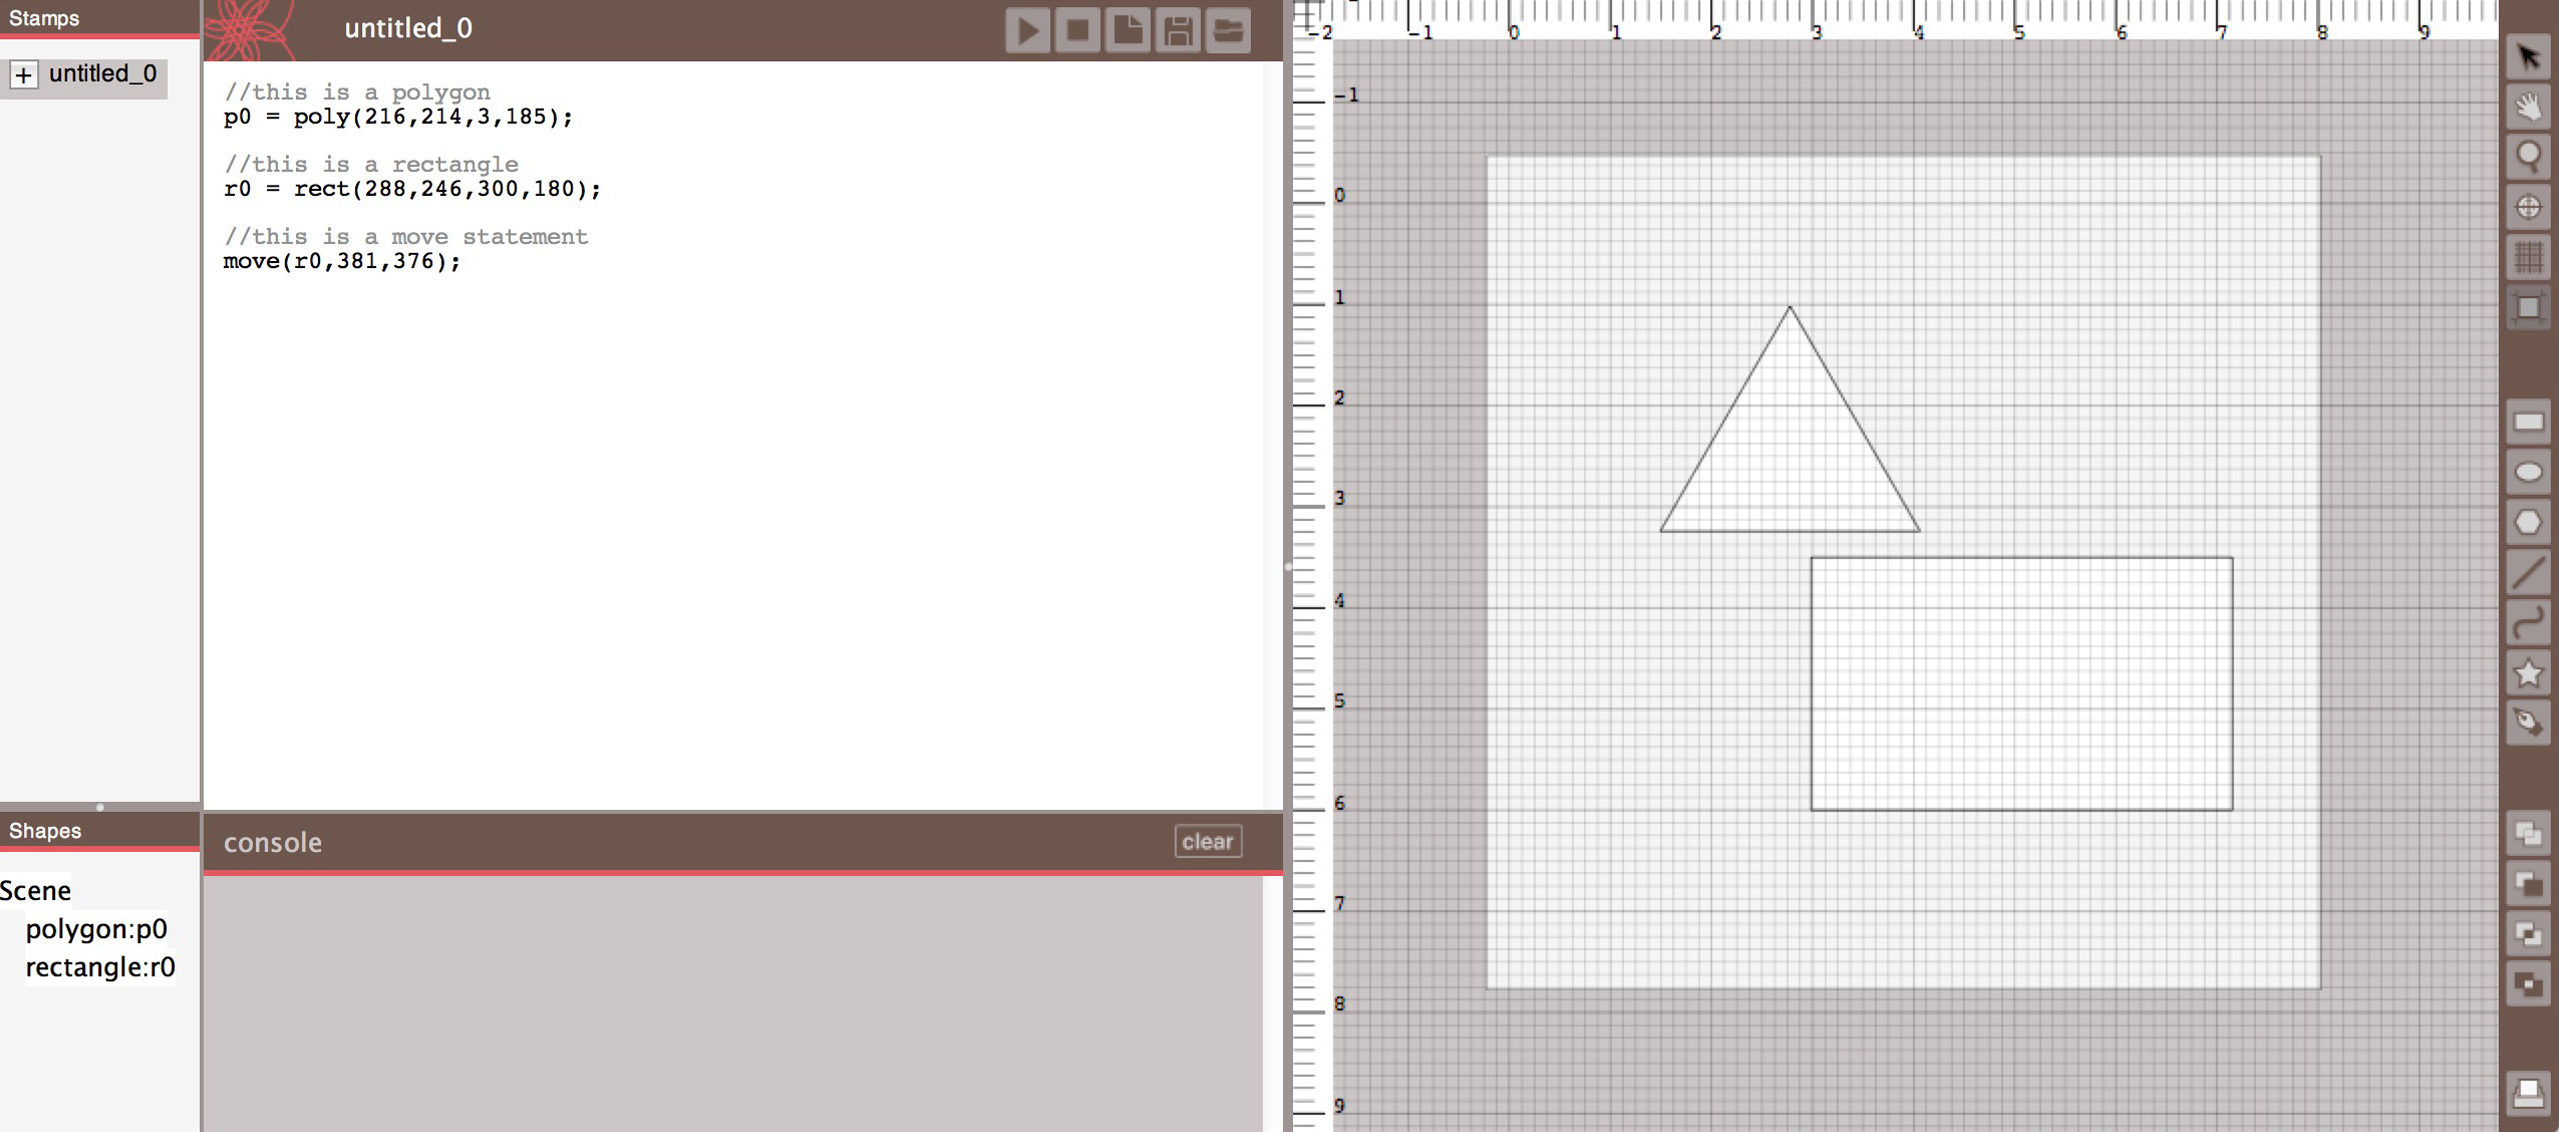
\includegraphics[width=\textwidth]{images/application_image_sm_content.jpg}
\caption{The DressCode Software)}
\label{fig:application_image}
\end{figure*}

\subsection{System Overview}
The DressCode application resembles a mash-up of a digital graphic drawing tool and a text editor. The interface is divided into two primary panels: a graphic panel on the right and a text editor panel on the left (figure:\ref{fig:application_image}). A designer may write and execute programs using the text editor; or they can draw and transform shapes using the mouse in the graphic panel. Each panel contains specific features and tools to enable these respective interactions. The text editor contains a console for output and error messages and a panel with buttons for compiling and running the current program. The design panel contains a re-sizable drawing board and grid with rulers corresponding to physical units (inches and millimeters), and pan and zoom tools to facilitate navigation. A toolbar on the right-hand side of the graphic panel contains a menu of drawing and transformation tools as well as contains a print button which allowing one to export their current visual design in vector format for output through printing, or 2-axis forms of digital fabrication (figure:\ref{fig:graphic_tools}).

\begin{center}
\begin{figure}[h!]

\includegraphics[width=\columnwidth]{images/graphic_tools.jpg}
\caption{The graphic drawing and transformation tools in DressCode (from left to right: selection and move tool, rectangle tool, ellipse tool, regular polygon tool, line tool, curve tool, SVG import tool, pen tool)}
\label{fig:graphic_tools}
\end{figure}
\end{center}
\vspace{-20pt}

The graphic drawing tools include regular shape creation tools and a pen tool for enabling the free-hand drawing of of irregular shapes. In addition to the drawing tools, the selection tool allows for individual shapes and groups to be manually selected and moved, and the boolean operation tools allow for the combination of two or more shapes into a unified form through a variety of polygon-boolean operators (union, difference, intersection and either/or). The interface also contains two additional panels, the stamp panel and the declarative view which are described in the correspondence~\ref{subsec:correspondence} and readability~\ref{subsec:readability} subsections below.

 DressCode contains a custom imperative programing language which supports conventional programming data-types, loops, conditional expressions and user-defined functions. Variables in DressCode are dynamically typed and identifiers can be assigned to data-types that differ from their original assignment.The language contains a subset of expressions which facilitate the drawing and transformation of 2D graphic geometric forms \textcolor{red}{add figure here to show syntax}. The language also supports math expressions and enables a variety of random noise generation methods. We describe the drawing API of the DressCode programing language and their relationship with the graphic manipulation tools at length in the following section. A note on terminology: for the remainder of this paper, we denote actions made in the graphic panel with the mouse as \textit{graphic actions}, and actions made in the programing panel by typing expressions as \textit{programmatic actions}. We also distinguish between two types of actions: \textit{initialization actions} denote programmatic or graphic actions which result in the creation of a new shape and \textit{transformation actions} denote programmatic or graphic actions which result in an existing shape being moved, rotated, scaled or otherwise altered.  


\subsection{Linked Representations In Practice}
Graphic tools and programing tools have separate affordances. Graphic tools are based on metaphors of physical drawing and manipulation with traditional media, and often represented by icons and symbols that reflect this. As a result, they can be intuitive or inviting to new users. Textual programing tools are traditionally less intuitive, but have the advantage of readily supporting complexity and automation in design, and are a natural fit for parametric representations. Because of these differences, combining computational and graphic design into a unified interaction raises many questions around interaction design: What forms of interaction best support the distinct affordances of graphic manipulation and programing? How should graphical organizational structures be reconciled with computational forms of organization? What rules dictate the resolution of inevitable conflicts between graphical and programmatic actions? How does the intended application of the software dictate the relationships between the two paradigms? To approach these to these questions, we developed the linked representations in DressCode around two primary design principles: Symmetry and Readability.We describe the latest state of the tool with respect to these principles. We wish to emphasize however, that this state was achieved though a series of tests with successive versions in our workshops. The workshops not only directed the iterations of the tool itself, but assisted in the clarification of the design principles behind it.

\subsection{Correspondence}
\label{subsec:correspondence}
The governing design principle in DressCode is correspondence between programmatic actions and graphic actions. For every shape that is initialized programmatically, a graphic element is generated in the graphic view. Conversely, for each graphic action, a corresponding programing expression appears in the text editor. The DressCode programing language syntax was developed to support the translation between graphic and programmatic representations. The drawing API is formulated on an Object Oriented Programming paradigm where basic shapes (points, lines, curves, polygons etc.) are initialized by calling the appropriate method and passing it a set of parameters designating its location and dimensions. If a shape is initialized graphically, its parameters are determined by the mouse gestures of the designer (where they click to determine the origin, and how far they drag from the origin to determine the dimensions). The method-type of the auto-generated expression that results from a graphic action is determined by the type of graphic tool that was used to create the shape, and the parameters determined by the graphically defined dimensions. Shapes are layered in a design in order of the designer's graphic and programmatic actions, with shapes that were drawn most recently appearing on top of those created earlier. %clarify this last sentence

Transformation methods, including moving, scaling, rotation, color and stroke changes, and shape booleans follow a similar structure to shape initialization. In the programing language, transformations are performed by either wrapping a shape-initialization expression in an a transformation expression, or by assigning an identifier to the shape, and then calling the transformation method with the identifier. Each graphic transformation tool corresponds to a transformation method in the DressCode language, enabling the auto-generation of an expression in the programing panel which contains as its first argument a reference to the shape which was selected and manipulated graphically. Throughout the design process, a complete representation of the current state of the graphic design is continually maintained in the programming panel. This representation allows programs to be shared and remixed easily; if the textual program from one design is copied and inserted into another designs' program, it will re-generate the exact design in the context of the new design. 

\subsubsection{Static and Dynamic Generativity}
Organizational structures are an essential component of CAD as a design grows in complexity. \textcolor{red}{need to re-work this section so it fits in with correspondence, or move it somewhere else} DressCode contains functionality to help people organize their code in the form of static and dynamic \textit{stamps}: graphically created functions that return shape primitives. Dynamic stamps are created by selecting a portion of code in a user's program and then selecting the dynamic stamp option from the menu. A dynamic stamp will package the selected code in a function with a name specified by the user. Static stamps are created by graphically selecting a single primitive or group with either the selection tool or the declarative view, and selecting the static stamp option. Static stamps translate shapes generated in random positions to explicit primitives, allowing users to save a specific instances of a generative design (see Figure \ref{fig:stamps}).
Stamps are listed in the stamp menu and can be added to a user's primary program by selecting the \textit{+} icon next to each stamp. The code of both static and dynamic stamps can be modified by the user as the code generated is human readable.

\begin{center}
\begin{figure}[h!]
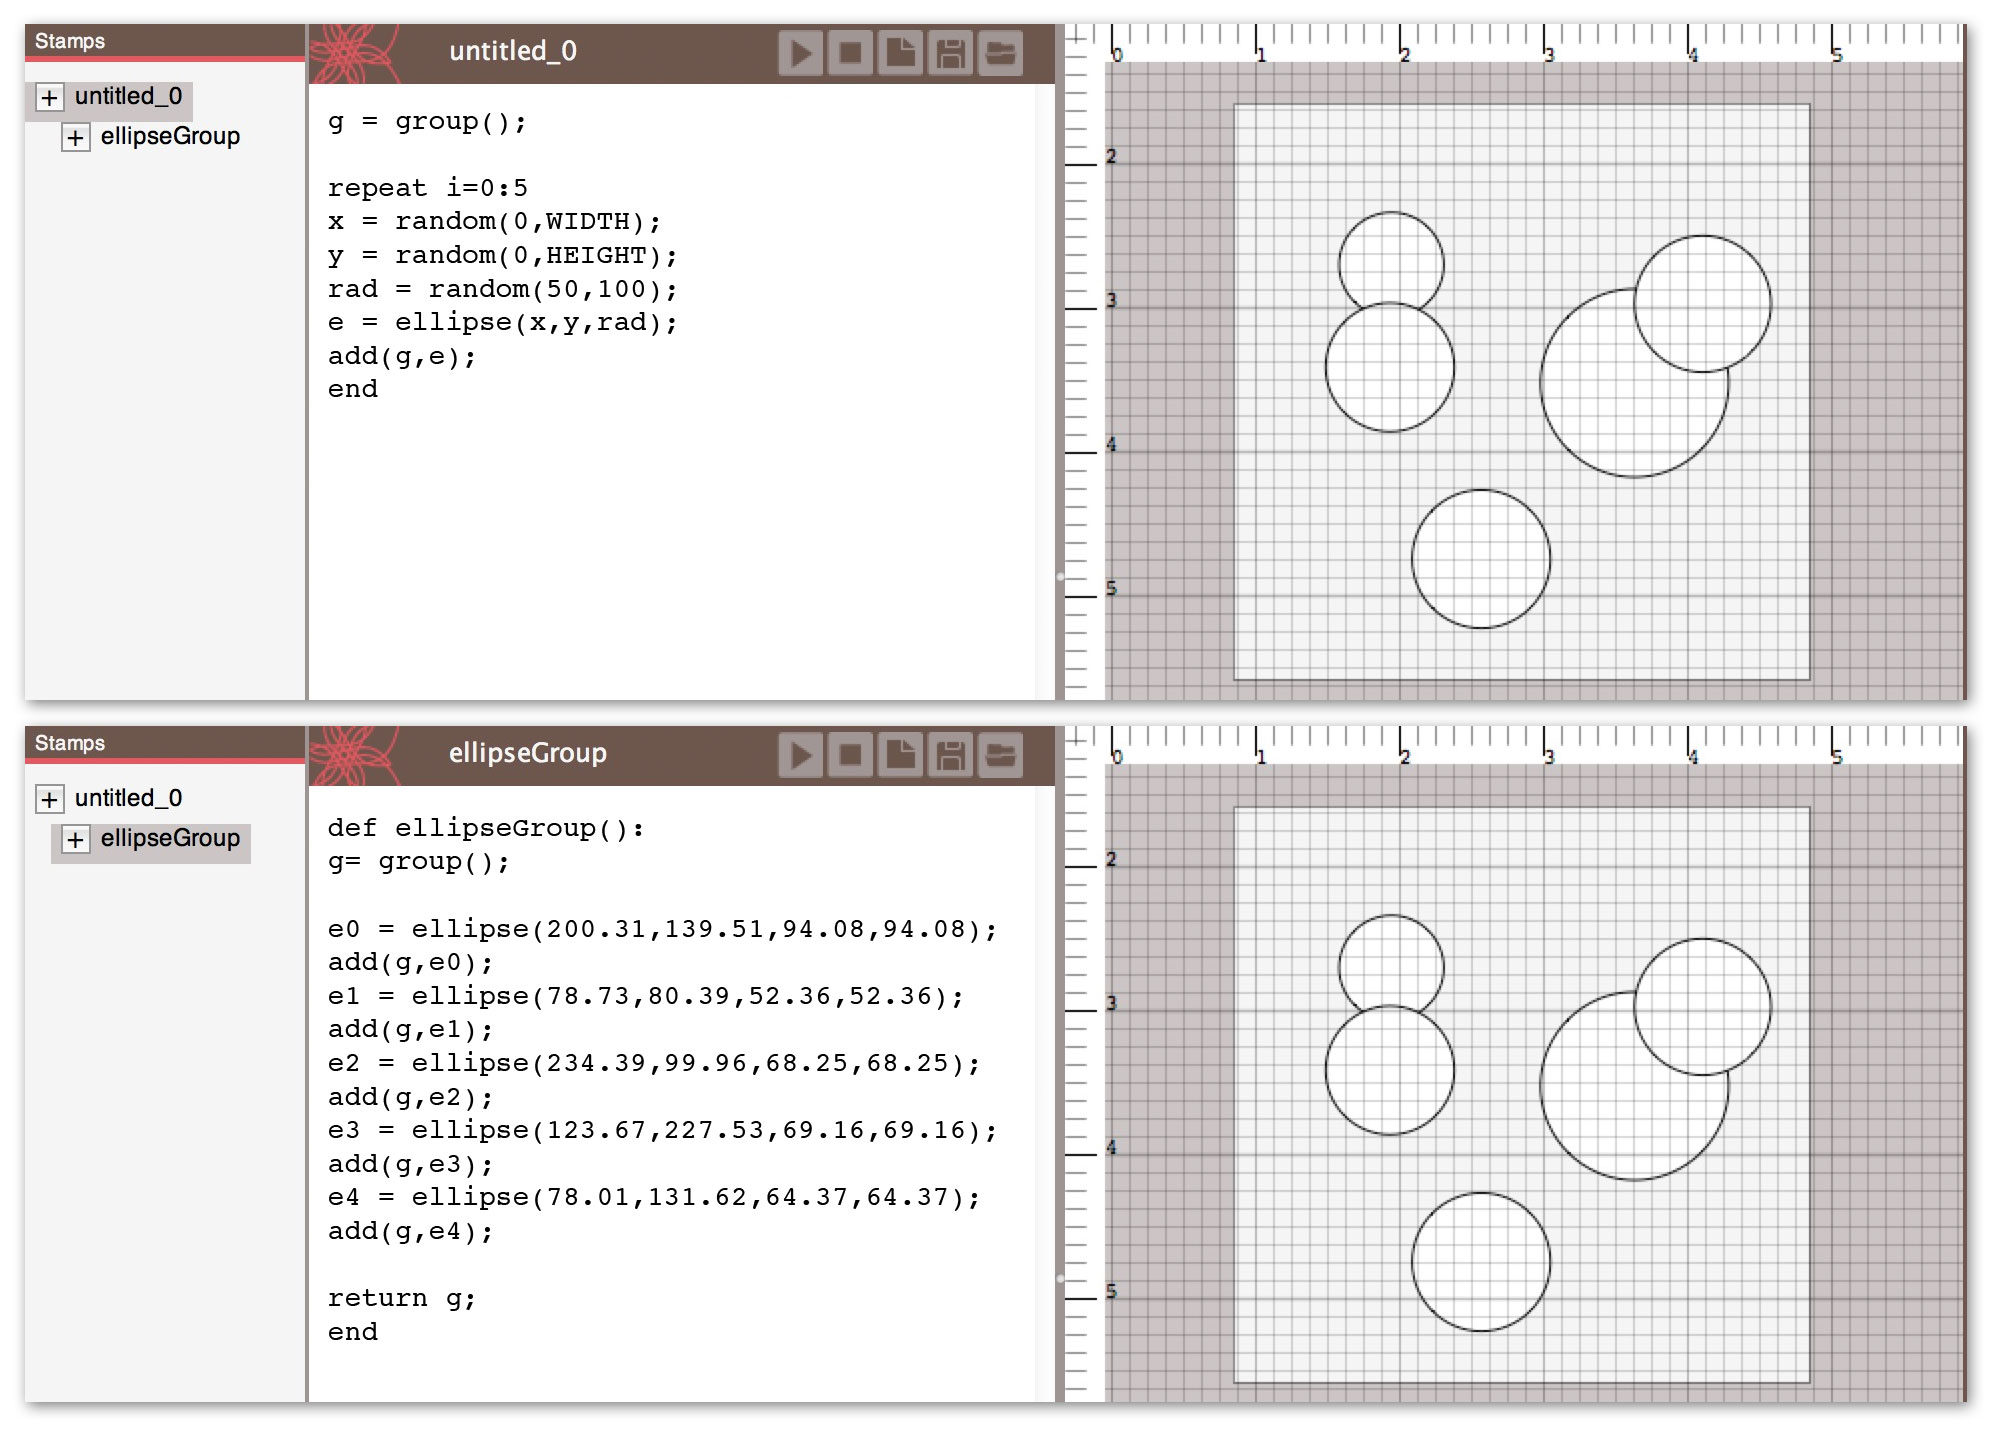
\includegraphics[width=\columnwidth]{images/stamps.jpg}
\caption{Static stamp functionality. (Top: User defined code which generates five random ellipses. The ellipses' positioning and size will change each time the program is run. Bottom: static stamp created from ellipses which will always return the same design.)}
\label{fig:stamps}
\end{figure}
\end{center}
\vspace{-20pt}

\subsection{Readability}
\label{subsec:readability}
As we discovered through our implementation, Symmetry between graphic manipulation and textual programing must be tempered by concerns of usability. Merely producing a textual expression that accurately reflects a graphic action does not ensure that the interaction will be interpretable to the designer, let alone useful to their design process. We therefore considered how we could design linkages between programmatic and graphic actions which were not only functional, but transparent, readable, and reconfigurable by young people. 

\subsubsection{Readable Edits}
First, we considered \textit{where} auto-generated expressions would appear within a program. For an initialization graphic action the programming expression will always appear below the last line in the program. If the designer performs a transformation graphic action however, the expression will be inserted into the line below the initialization of the selected shape, or below the last transformation expression for the shape. This structure ensures that the modified program will reproduce the correct order of operations when run, but also provides a form of organization to auto-generated statements. Naturally, in the process of manually writing code, the designer may consciously or unconsciously write expressions in a manner that deviates from this organization. Fortunately, manual edits by the designer will not prevent the ordering mechanism from functioning for successive graphic actions. More importantly, the consistent, simple rule-set for auto-insertion enables the designer to anticipate where expressions will be inserted into their code, which is essential to allow them to make edits as a program grows in length and complexity.

\subsubsection{Readable References}
Like many existing programing languages, DressCode gives the developer flexibility in how they reference program are referenced. The DressCode language enables methods to be nested within one-another, so there is a degree of ambiguity for how a designer may use identifiers in their code. As a result, it was necessary to evaluate \textit{how} shapes should be referenced when transitioning between programmatic and graphic representations. Here we also advocated for an approach that would make the design "readable" for new programmers. All initialization graphic actions produce programmatic expressions that are automatically assigned an identifier. Subsequent transformation graphic actions will produce programmatic expressions that reference the auto generated identifier on the following line. This produces code that while requiring more lines, is arguably more readable than a nested chain of expressions. If a shape that was programatically initialized without an identifier is transformed graphically, DressCode will recognize the distinction and resort to wrapping the initialization expression in the appropriate transformation expression. If the designer re-assigns or modifies the identifier of a shape through a programmatic action, future graphic actions on the shape will recognize this modification and use the new identifier.   

\subsubsection{Readable Design Steps}
 It was important to us that the steps used to arrive at a design were also readable. Because the DressCode programing language employs an imperative paradigm, designs are represented as a series of the designer's actions, rather than a declarative state. We structured the auto-generated statements so that the programmatic expressions reflected the order of steps a designer made in the graphic interface. DressCode takes a verbose approach to generating programming expressions. For example, when a shape is moved with the move tool, a textual move expression is inserted into the designer's program. For all subsequent moves following the first move, rather than generate a successive string of additional move statements, the move expression is updated to reflect the new coordinates of the shape. However, if another tool is used to alter the shape, or a programmatic expression is manually inserted by the designer following the move statement, future actions with the move tool on the same shape will generate a new move statement, which will be subsequently updated until another tool is used (see Figure \ref{fig:auto_generated_code}). This same logic applies to all other transformation tools in DressCode. We chose this structure, because it allows the program to preserve the designer's actions in the graphic panel as a series of discrete steps, thereby providing an opportunity for the program to also serve as a means of reflection and evaluation on one's practice and design intentions \textcolor{red}{I feel like this section is maybe repetitive of what I say in the correspondence section}. 

\subsection{Declarative Representations}
Although DressCode relies on an imperative paradigm, we recognized that a state-based representation could provide a useful means of illuminating the connections between the visual design and the textual program. Specifically, it was important to help a designer determine what code in their program was affecting specific shape in their design. Contemporary programing environments now frequently employ debug tools that allow the user to step through their code in an effort to decipher its effects. Similarly many code editors contain declarative listings of all of the methods and identifiers in a class, providing an alternative means of navigating one's code. We combined these tools in a way that is specific to a tool for programing and graphic drawing. DressCode features a declarative view which contains a listing of all primitives in the current design. Child primitives are nested within their parent groups. When selected in the declarative view, the primitive is selected and highlighted in the design view, and the line where the primitive was last modified in the text-editor is highlighted (see Figure \ref{fig:declarative_view}). The declarative view provides visual feedback on how elements of a design connect to the program, and provide a practical selection technique for complex designs.

\begin{center}
\begin{figure}[h!]
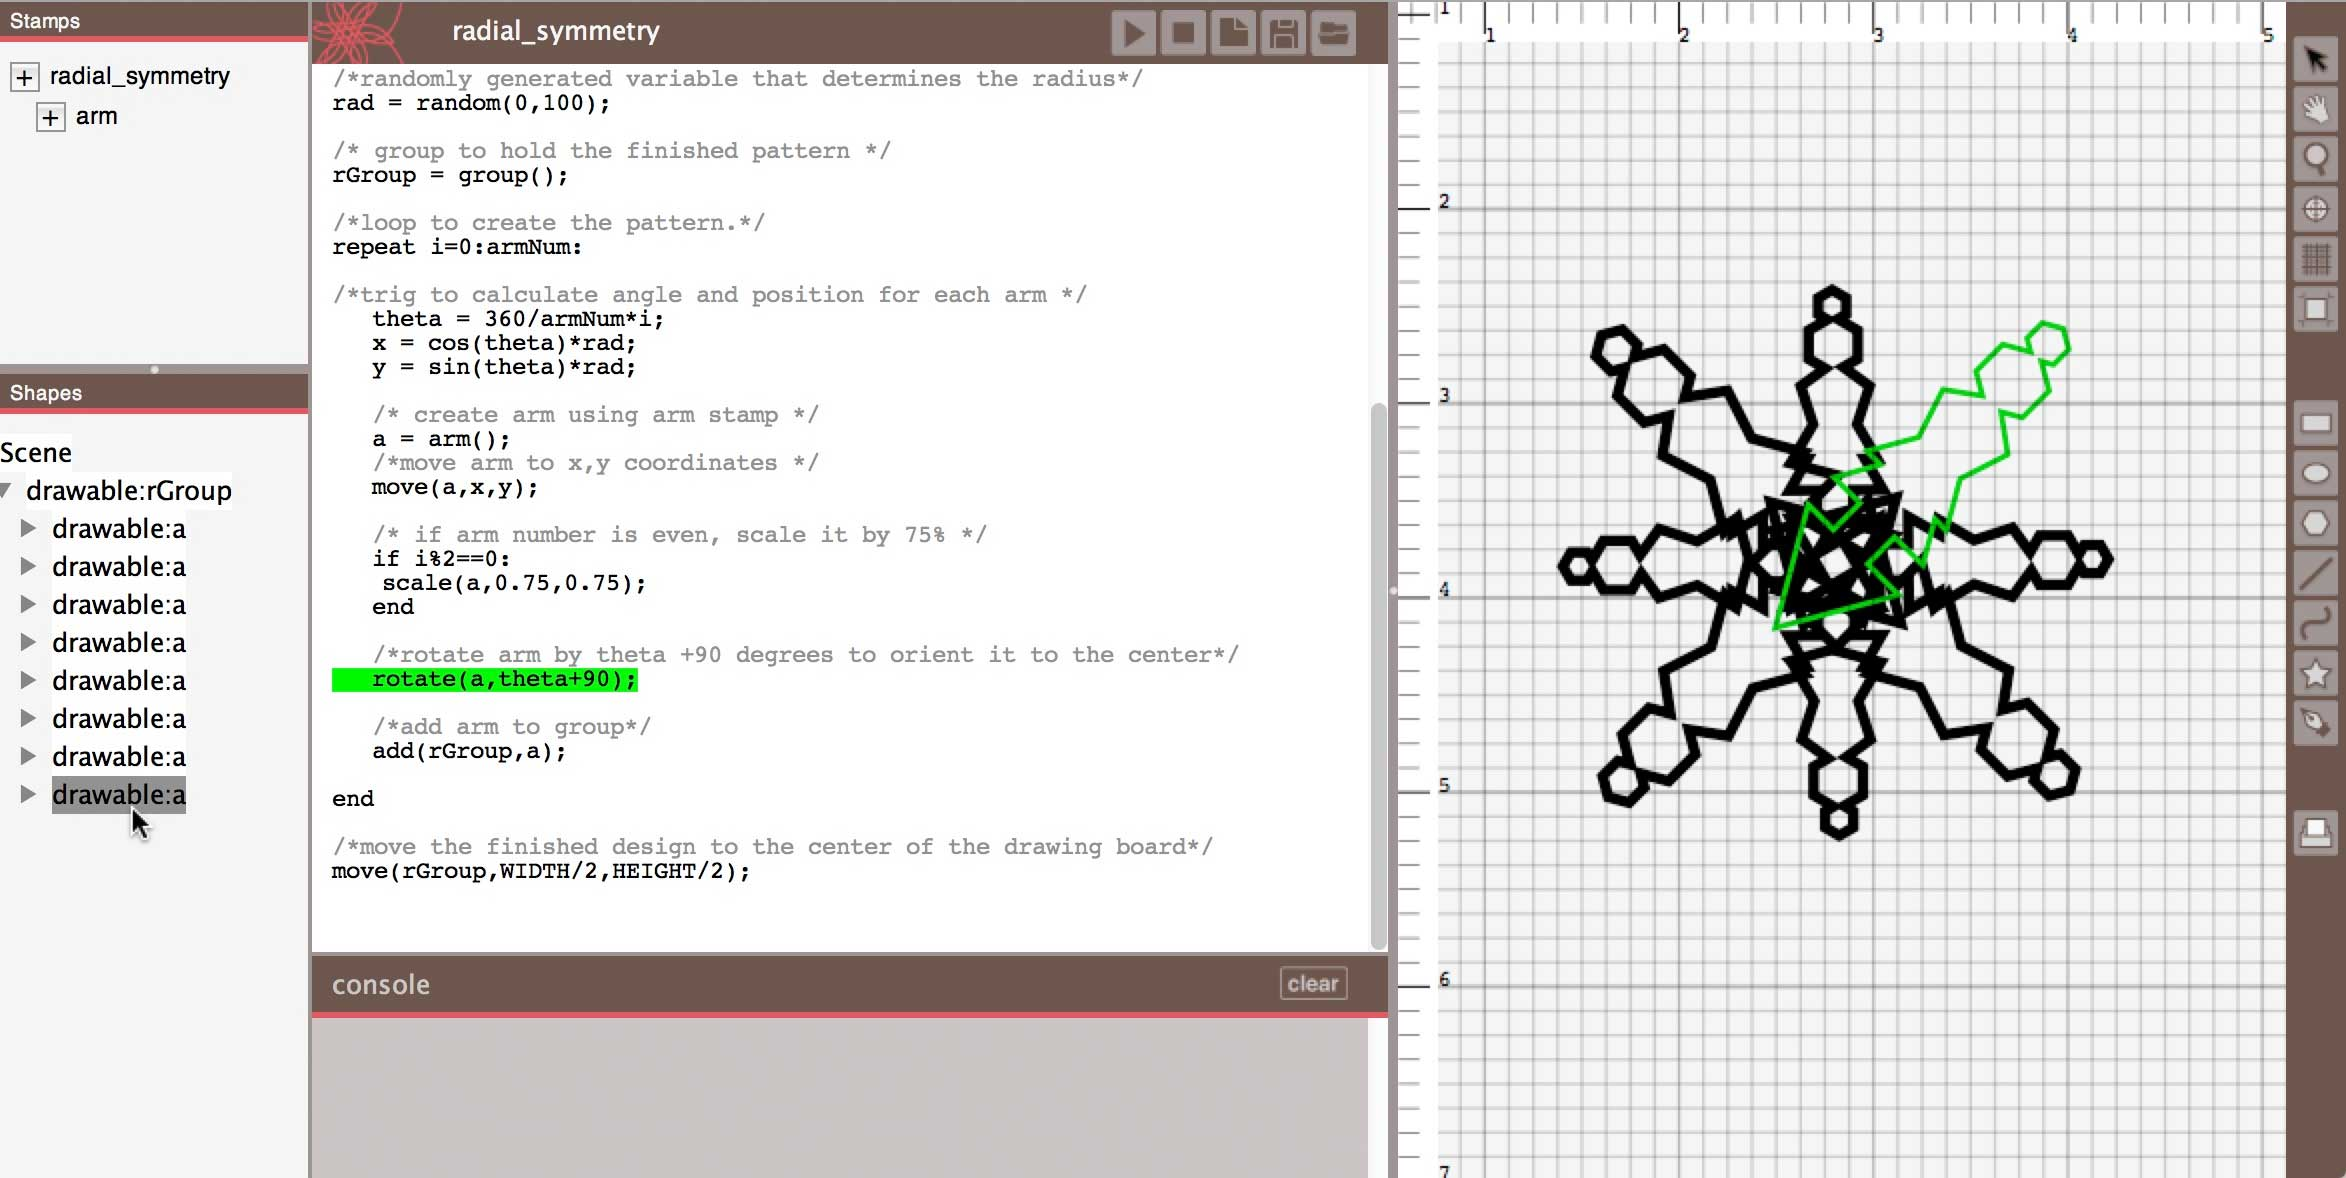
\includegraphics[width=\columnwidth]{images/selection_mechanism.jpg}
\caption{Declarative view with selected primitive}
\label{fig:declarative_view}
\end{figure}
\end{center}
\vspace{-20pt}



\section{Workshops}
\textcolor{red}{taken from prior paper, need to condense and make specific to this version.}
We evaluated DressCode with young people through two workshops. Both workshops focused on using DressCode to produce wearable artifacts. The preliminary study consisted of a one-day workshop in which participants designed and fabricated leather wrist-cuffs. The long-term evaluation was conducted through a four-day workshop, divided between two consecutive weekends, in which participants created computational designs and screen-printed them onto t-shirts. 

\subsection{Evaluation Methods}
The participants' experiences were evaluated through written surveys, interviews and group discussions. The surveys were aimed at understanding participants’ prior attitudes towards programming, design and craft, their interest in and attitudes toward programming and design, and their engagement in and enjoyment of the workshops. Pre-workshop surveys focused on participants’ previous experience and attitudes towards programing, craft and design, how personally useful they felt programing to be, and how good of a tool they found it for creativity, personal expression. They also asked students to describe their views on design, programing and craft practices as they related to referencing examples, learning from other's work. Post-workshop surveys contained attitudinal questions that were matched to the pre-surveys. In addition, post surveys contained a range of written questions asking the participants to describe their design process, their opinion of the success of their projects and their experience using DressCode. Interim surveys were also administered during the primary workshop following the first two days, and questioned the participants on experiences with DressCode programing language and graphic tools and how the combination of features hindered or supported the design process.

In-person interviews were conducted with the participants in the preliminary workshop. These interviews lasted an average of 10-20 minutes and were audio recorded and transcribed. During the interviews, the participants were asked to describe their artifact, and talk about the process of conceptualizing, designing, and producing it. In the primary study, participants were engaged in three group discussions at the start, middle and end of the workshop which were similarly recorded and transcribed. The discussions examined participants' design process, experience using DressCode in combination with craft practices, and ideas they had for modifying or augmenting future activities and software tools. In both the interviews and discussions, participants were also asked to describe what they enjoyed, what was difficult for them, and what they felt they had learned through this process. Survey results, verbal interview and discussion responses and project outcomes were analyzed to determine how they connected to the primary research questions we associated with algorithmic craft in the introduction. We also used this information to identify repeated and notable elements of participants experiences, and formulate a set of criteria for future development in algorithmic craft.

\subsection{Preliminary Study: Wrist cuffs}
The wrist cuff workshop was conducted among 10 young adults, aged 15-17, 20\% male and 80\% female. Of those surveyed, three participants had prior experience with Scratch, and two had worked briefly with the Arduino programming environment in a prior workshop. All participants said they had some prior experience in art, design, or craft. Prior to the workshop, 60\% of the participants indicated that they did not feel comfortable programming on their own; however, the majority indicated they were interested in learning more about the process. 

During the workshop, participants used DressCode to design a pattern for a wrist cuff, laser-cut their patterns into leather and assembled the finished wrist cuff by hand. The computational design in the preliminary study was structured around radial symmetry, and the majority of the resulting artifacts featured patterns that were derived from radially symmetric structures. Participants wrote their own radial symmetry algorithms, and were then provided with a template in DressCode that automatically clipped their designs to the dimensions of a cuff sized to their wrist. Participants were given two hours to design, and 3 hours to fabricate and assemble their piece.

\subsection{Preliminary Results}
Each participant in the preliminary workshop was successfully able to use DressCode to produce a unique leather cuff. The design approaches and aesthetics of participants varied greatly. Some cuffs were geometric, some were floral, and many styles were difficult to link back to the original radial algorithm. Each participant was able to write their own radial symmetry algorithm in the initial lesson and produce a variety of patterns with it. During the design portion, several participants extended the radial symmetry algorithm with additional design elements, however most participants designs relied exclusively on structures that were possible with radial symmetry. Eight of the participants said they planned to wear the bracelets they created, and two indicated that they planned to give them as gifts. A comparison of the
pre-and post-workshop surveys demonstrated increased comfort with programming as a result of the activity. After the workshop, more participants indicated that they thought programming was a good tool for personal expression and design. All participants stated that they believed they could use programming to make things that were beautiful, whereas several had disagreed with this statement before the workshop. All participants unanimously identified the programing portion as the most difficult component of the workshop, however the majority said they were interested in continuing to learn more about computational design for craft applications. 

\subsection{Design Revisions} Here is how we changed DressCode between workshops

\subsection{Primary Study: Screen Printing}
The screen printing workshop was conducted among 7 young adults, aged 13-17, and one older participant, aged 21. Three participants were male and five were female. Participants for the workshop were deliberately selected to represent a range of programing and design experience. Two participants, (one being the oldest participant), were relatively experienced programmers, having worked extensively with java, python and lua. Two participants considered themselves intermediate to novice programmers with basic experience in Scratch, HTML, Python or App Inventor. Two other participants had prior exposure to Scratch, but had not worked with it extensively. One participant had no programing experience, but was interested in learning. Participants also varied on their prior experience with digital design software. Two indicated that they had no prior experience with design software, two had previously used the graphics editor in Scratch, three had used Adobe Illustrator or Photoshop, and one person was shown Solidworks in a summer course, but had limited experience with it. The majority of participants indicated they had a variety of prior crafting experience, including making jewelry, basic woodworking, sculpture and origami. One person had screen printed before using vinyl cut stencils. Interestingly, one participant also identified soldering a electronic synthesizer kit as a craft activity. Only one participant stated that they had no prior craft experience.

Because the screen printing workshop occurred over a four-day period, it provided the opportunity to explore the computational design process in DressCode in greater depth, and allowed for the participants to engage in a more complex craft process: photo-emulsion based screen printing. Prior to the workshop, we had participants select t-shirts in a size and color of their preference. The first session of the workshop, we introduced participants to the concept of generative design, and demonstrated techniques for incorporating random elements into a pattern or graphic. We introduced participants to textual programing in DressCode by guiding them through writing their own random walk algorithms that produced patterns composed of lines. Following this, we explained the functionality of the graphic drawing tools, and had participants modify their random walk patterns by incorporating shapes they created graphically. The following session we discussed the general process of screen printing and demonstrated several other forms of generative design first we provided them with images of sample designs and had them work in groups to write a set of instructions that they thought would re-produce that design. As a group we discussed their results, and then demonstrated examples in DressCode that would produce similar results to the sample designs (figure:\ref{fig:example_designs}). Participants were then provided with the design task of creating a computational design to screen print onto a t-shirt they would want to wear, and given 3 hours of open design time with the option of modifying the examples we provided, working off of the original random walk pattern they had created the first day, generating a design from scratch, or working with an instructor to come up with additional design ideas. The following session participants prepared their screens for screen printing, by stretching the screen material over the frames in groups and applying the photo emulsion to their screens. Afterwards, participants were given 2.5 hours of additional open time to complete their designs. Participants laser-printed their finished designs on transparencies, which the instructors exposed on the screens overnight (figure:\ref{fig:screen_printing_process}). The final session, participants practiced printing with their designs on test materials, and then printed onto their t-shirts.

\begin{center}
\begin{figure}[h!]
%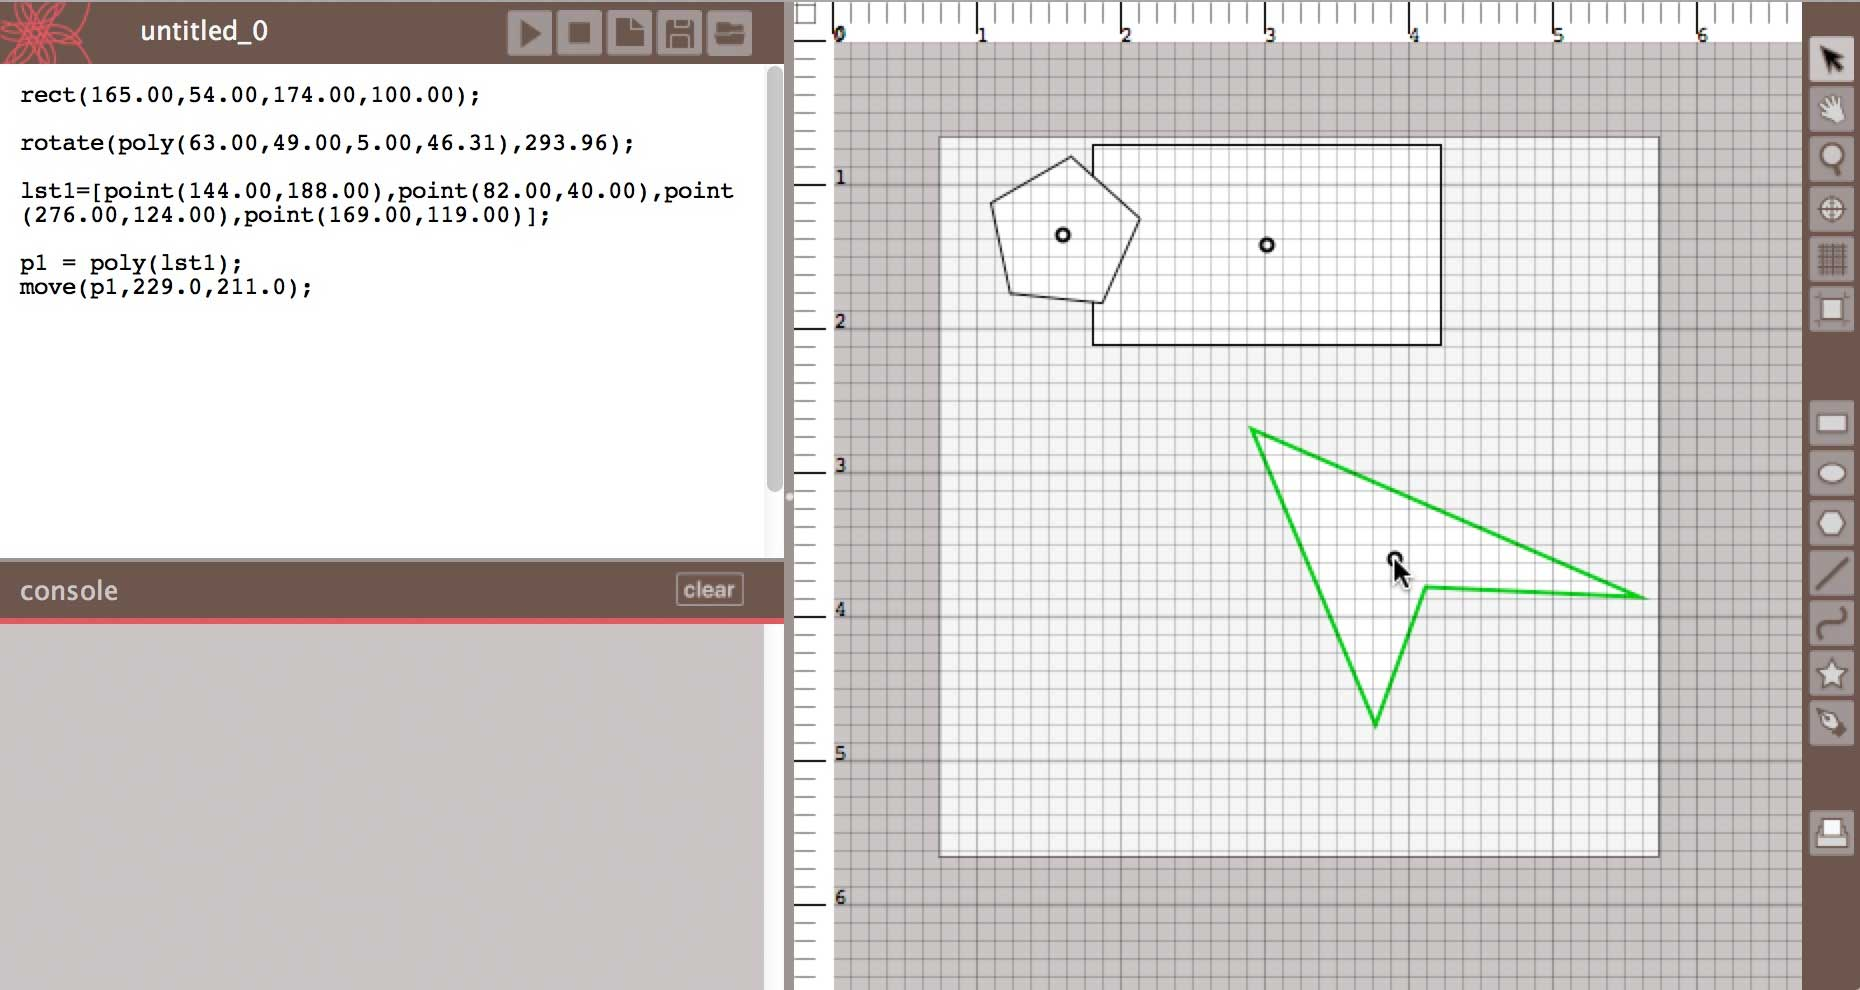
\includegraphics[width=\columnwidth]{images/auto_generated_code.jpg}
\caption{Sample Designs and corresponding examples in DressCode}
\label{fig:example_designs}
\end{figure}
\end{center}

\begin{center}
\begin{figure}[h!]
%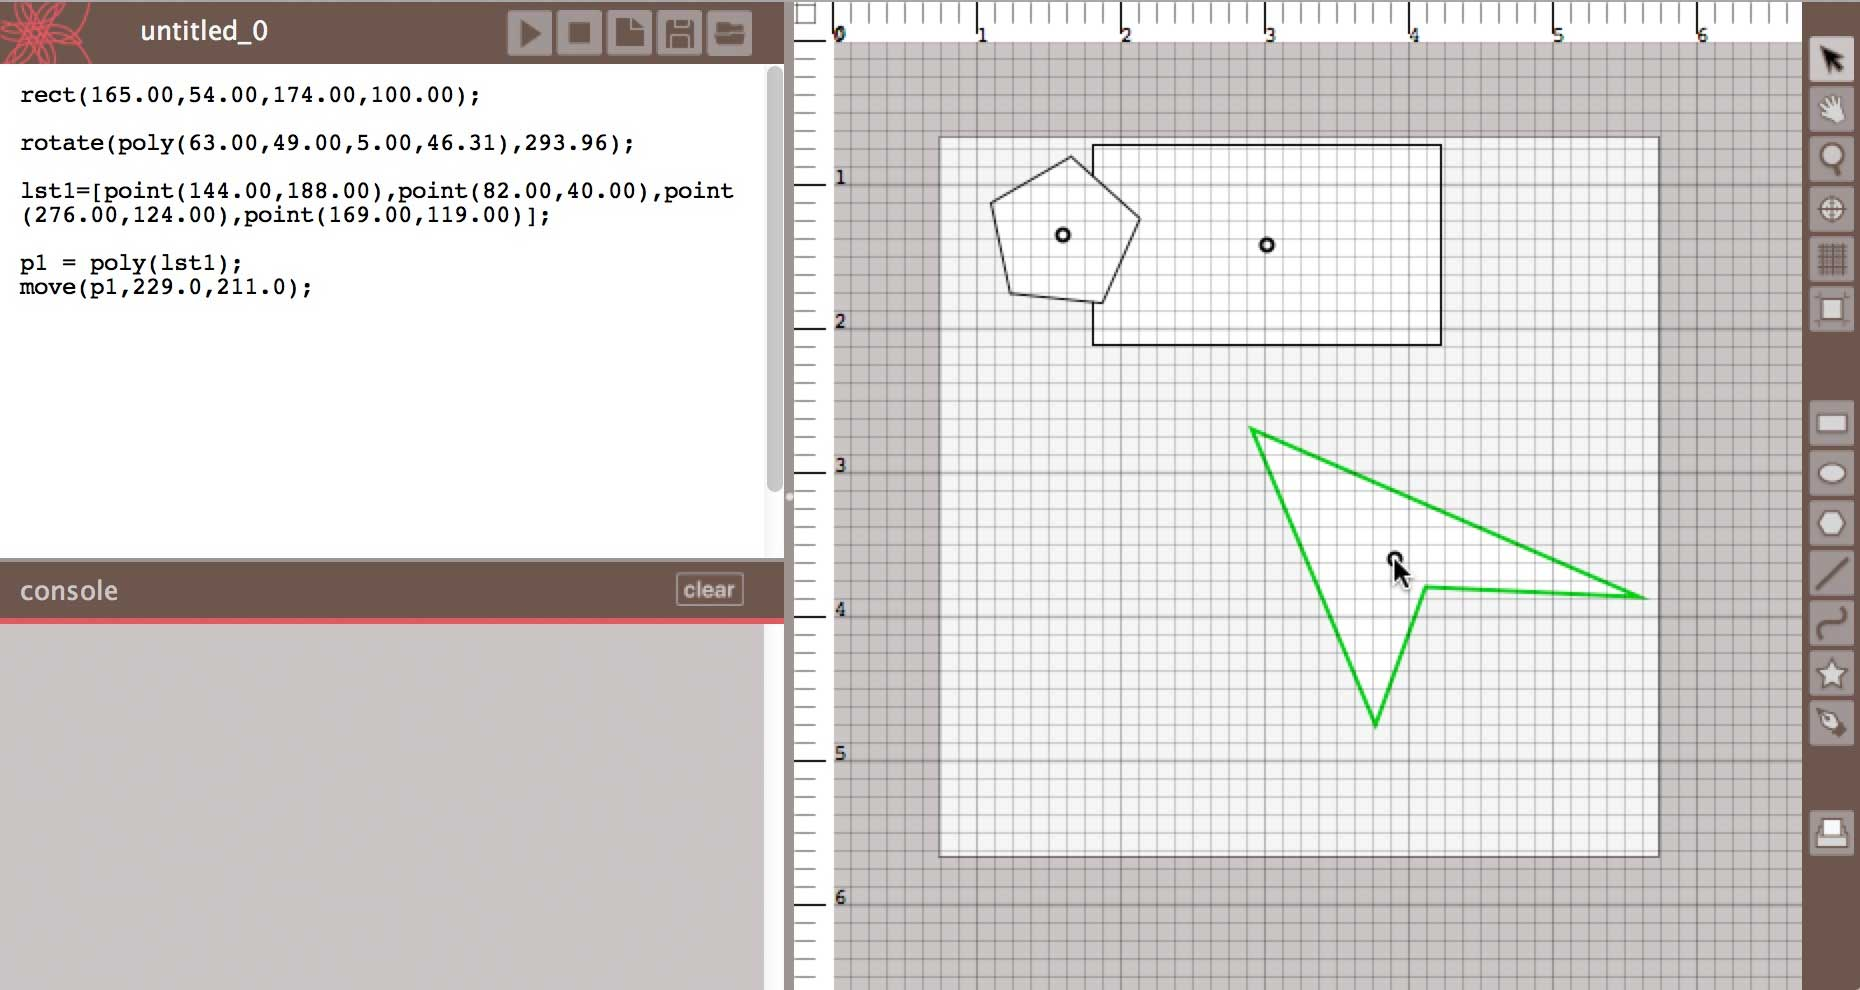
\includegraphics[width=\columnwidth]{images/auto_generated_code.jpg}
\caption{Screen printing process}
\label{fig:screen_printing_process}
\end{figure}
\end{center}

\subsection{Screen Printing Results}
Each participant in the primary workshop was successfully able to use DressCode to produce a design for their t-shirt. The design approaches among the participants varied. Two participants created designs that were derived from their random walk algorithms, one participant created a pattern by combining two of the example patterns and making adjustments, and one participant worked solely by modifying an example. Other participants designed patterns independent of the examples, including a generative landscape, a geometric spiraling pattern and a complex radial pattern comprised of overlapping lines. The screen printing process was extremely popular among the participants. Each person was successful in creating their screen, transferring their design to the screen and printing to the shirt, although one participant had to re-expose his screen because of errors in applying the emulsion. Several participants not only printed to the provided shirts, but also brought in additional garments to print on for friends and family. The participants requested to keep their screens following the workshop, and stated on the survey that they planned to continue making prints for themselves and others. All participants indicated that they planned to wear their shirts, and two participants contacted us via email following the workshop thanking us for the experience, and requesting tips on how to properly care for their garments. 

From survey data and group discussions, 3 participants found the screen printing portion to be most difficult, 3 found the programing to be the most difficult, and one was equally challenged by both portions. An evaluation of the pre, mid and post-workshop surveys demonstrated that following the screen printing, participants attitudes towards programing, design and craft, changed from what they were after the computational design sessions. In the majority of cases, this change was positive; participants indicated greater interest in learning programing in the future, a stronger belief that programing was a tool that they could create things they would use in their daily life, and greater comfort in programing on their own following the craft activity. Six of the eight participants stated that they liked their design better after printing it, and all participants stated that the process of screen printing had given them ideas for additional designs they would like to create with DressCode. For a minority of participants however, the difficulty of the craft portion seemed to result in a slightly diminished interest in combining craft and programing, and a diminished interest in craft in general. Participants were positive about the graphic tools, although they requested that their functionality be extended to incorporate a greater range of transformation methods (rotation, scaling, and boolean operations). All 8 participants said they would be interested in using DressCode for another activity, and the majority indicated that they would like to combine computational design with 3D printing.

\section{Discussion}

\subsection{Diversity in design practice}
Computational design tools in the hands of novices can lead to a diversity of design practices: 
1)intuitive form allows for scaffolding the process of learning programing.
2)Flexibility in the degree in which people rely on computational or graphic methods
3)Design outcomes themselves are impressive, and noteworthy for their aesthetic qualities of blending hand and computational aesthetics.

 This points the potential creative openness of linked representations as computational design tools, and suggests that even more diverse approaches may result from longer design sessions. Second, because all of the approaches incorporate a significant degree of computation, it seems evident that computational design methods are relevant and appealing to young designers. As further evidence of this, when we asked the group if they would have preferred to participate in a similar workshop where designs were drawn by hand, or drawn w
Responses from the participants regarding the use of DressCode affirmed our attitude that the tool was accessible for novices. Before the graphic tools were formally introduced, several participants independently started experimenting with them on their own.  When asked to describe the tool structure, one participant responded"
\begin{quotation}
\textit{You find a tool, you draw on the canvas and it shows you the code, that's basically it.}
\\Participant Z
\end{quotation}
Several people also indicated that the graphic drawing tools also helped them to better understand the process of writing their program. As articulated by another participant:
\begin{quotation}
\textit{I think that having the drawing tools and having it also show the code there makes it so that you can see as you're doing it. [By] having a graphical side and having it auto update the code, it can show you that you want to work with the code you're learning as you're using the GUI. So that people could try and say ok, if I can't do something with the graphical tools, let me try and manipulate the code. And then you already have some understanding because you've been using the graphical tools and it's been appearing over there the entire time.}
\\Participant B
\end{quotation}
As designers, we find these responses to the tools as intuitive and understandable to be encouraging. As researchers, we find it more pertinent (and more interesting) to speak to the types of design practices our tool engendered. In the workshops, we observed three general design approaches. 1) emphasis on programmatic methods: participants who used the graphic drawing minimally, almost exclusively relying on generating and transforming methods computationally. All of the participants in the first workshop fit this category (due to the lack of extensive graphic drawing tools), as well as three of the participants in the screen printing workshop. 2) Programmatic manipulation of provided graphic elements: two people in the screen printing workshop used programming expressions to manipulate pre-existing graphics that had been provided in examples. 3) Equal use of graphic drawing and programmatic manipulation: Three people in the screen printing workshop used the graphic drawing and transformation tools in equal proportion with programmatic methods.

These three approaches lead us to three conclusions. First, we are encouraged by the fact that diversity of design practices emerged within a relatively short time-period of using the tool. This points the potential creative openness of linked representations as computational design tools, and suggests that even more diverse approaches may result from longer design sessions. Second, because all of the approaches incorporate a significant degree of computation, it seems evident that computational design methods are relevant and appealing to young designers. As further evidence of this, when we asked the group if they would have preferred to participate in a similar workshop where designs were drawn by hand, or drawn with non-computational digital design tools, all but one answered that they either preferred the combination of the two forms, or at the very least, appreciated the option of using programming in their design:
\begin{quotation}
\textit{I think combine them (computational design and hand-drawing). I could go for either one, or both, it doesn't really matter because they're both fun.}
\\Participant M
\end{quotation}
\begin{quotation}
\textit{The important thing I really feel about DressCode is you can turn things like ''random". These are drawn [gesturing to a graphically drawn element of his design] and these are from the programing part [gesturing to the repetition of them] ... but in [Adobe] Illustrator it's just drawing. You can't have everything.}
\\Participant Z
\end{quotation}
The valuing of randomness and generativity was also evident in the screen printing designs themselves, where 5 out of 8 incorporated some form of noise in the design process. 

Finally, we saw aesthetically distinct designs emerge from the linked representations in DressCode. The participants who relied on a balance of graphic and programmatic design tools produced aesthetics which featured repetition generativity and complexity, however they were distinguished by the presence of graphic elements that were clearly attributable to the style of their individual creator. The graphic tools enabled the designers to computationally alter hand-drawn forms, producing pieces that contained imperfect, irregular forms in direct conjunction with computational aesthetics. Furthermore, this imperfect aesthetic was deliberate. During one critique session, the creator of the heart t-shirt explained to another participant that he had deliberately chosen to draw a irregular heart form, even though he realized it was possible to computationally create an assortment of perfect, regular hearts. As designers ourselves, we were incredibly excited by the diverse visual qualities of these hand-drawn/computational hybrids (to borrow a term from Zoran \cite{zoran_tochi}), and we consider the development of a more nuanced palette of hand-drawing graphic tools and mechanisms (perhaps a tablet an stylus), as a worthy next step of exploration in this field, enabling evidence of the human hand to be supported by, rather than eliminated by computational tools.

\subsection{Tensions in creating abstractions }
Through their analysis on ways design choices impact usability in hardware construction kits for novices, Blikstein and Sipitakiat argue that age appropriate design is important when introducing unfamiliar technologies to children \cite{blik}. When abstracting lower-level functionality of the tool, it is inevitable that people's design processes will be effected. By evaluating the tool in a long-term design process there is a greater opportunity to gain insight on how abstractions should be structured to maintain the accessibility while preserving features that are important to the target user-group. 

When we discussed people's experience with DressCode, participants not only described additional graphic tools they thought would be useful, such as a better curve tool, a shape scaling tool, and most prominently an eraser tool. More revealingly, they also talked about how they thought these tools should correspond with the programming environment. Here two participants discuss how they envision an eraser tool being implemented.

\begin{quotation}
Participant Z (Talking about erasing graphically): \textit{So if you erase one line, it becomes two lines...so it's going to generate the code for two lines.}
Participant M: \textit{No like if you drew a line with the sidebar, and then you decided you didn't like, you don't have to go to the code, erase it and press play, you could just take the erase tool, click on it and then it goes away.}
Participant Z:  \textit{No, what I mean is like if you just wanted to erase half..}
\end{quotation}

One participant in this conversation is advocating for a simplistic interaction, the ability to click on a shape graphically, and have both the line, and the code that generated be removed from the design. THe other is advocating a more complex editing functionality from the eraser- the ability to spawn new programing statements and create new shapes. 

People had similar discussions about the degree to which the creation of random distributions should be a graphic or programmatic. One participant wondered if he could have the software store the randomly created values for a specific program, and then have a graphic button that enabled him to reset these values to new random numbers when necessary. Other people stated that they would have found it useful to have graphic tools that enabled them create random groups of objects by pointing and clicking with the mouse. Other people strongly disagreed with this idea, stating that they felt this would take away from the process.

\begin{quotation}
 Well that would kind of take away from the programing part of it, because you’d be trying to turn everything into a UI, so it'd be like illustrator.
 \\Participant Z
\end{quotation}

The tensions present in these comments demonstrate the complexities in developing design tools for novices. The automatic inclusion of features that seem simple, such as an eraser tool may in fact lead to inaccurate assumptions about the design objectives of the people using the tool. Furthermore even when designing for novices, choosing the simplest interaction may not always be the best option if it trivializes the idea behind the interaction. Relegating random distributions to a pre-defined set of graphically selectable icons may make them more accessible for immediate use, but it could also prevent a designer from understanding or experiencing the opportunities afforded by structured forms of generativity in a design. 

\subsection{Designing Experiences to support a range of objectives and interests}
People approach tools and activities with different motivations. %deal with this partWhether performed by experts or novices, individual approaches to design are incredibly subjective and diverse \cite{learning_in_design}. 
Their response to the experience will be greatly effected by how accommodating the activity or tool was of their personal interests. In talking with people about what was most important to them in their experience using DressCode, people described a surprising range of different values. Some people appreciated the opportunity to create a unique artifact, as illustrated by this young woman who talked about her wrist cuff design:
\begin{quotation}
Youth Participant C: \textit{You can't find it at American Eagle. I buy a lot of my bracelets there, and you can't just go there and find this. I think it's cool if someone were to say ''Oh where did you get that from?, You can't find it." (Laughs).}
\\Interviewer:\textit{You can say that you made it yourself, you love how it's unique?"}
\\YouthParticipant C: \textit{yeah}
\end{quotation}

Other people talked about how they enjoyed the opportunity to produce something that was motivated by personal considerations:
\begin{quotation}
\textit{Usually when you make something you're making it like ''oh I hope society likes this" but this was about self satisfaction, so I don't have to take into consideration someone else's opinion.}
\\Youth Participant S
\end{quotation}

Whereas others saw benefit in engaging in computer programing for the first time.
\begin{quotation}
\textit{``[The] computer programming was enjoyable for me because I had wanted to do it before but never had the chance. So this workshop gave me exposure to something that I wanted to do for a while and I totally loved it."}
\\Youth Participant 092297m (survey)
\end{quotation}

We also found that some people valued the opportunity to learn a craft process, and that this experience added an extra value to the designs they had created computationally:
\begin{quotation}
\textit{I feel as though maybe like when you're programming stuff, you're on the computer but you're not using any physical work, but when you're screen printing there's the manual labor involved, so when you actually get something right it's I guess more gratifying, since you put hard work [into it]... Well you do put hard work into programming, but it's more a thinking thing, not actual physical labor.}
Participant L: \textit{After all this hard work, you have this (pointing to the t-shirt she is wearing)}
\\Participant R: \textit{It lets you take pride in it.}
\end{quotation}


In many forms of youth engagement in programing, we believe there is an inordinate emphasis is placed on learning computational concepts, rather than supporting diverse and subjective experiences. Brennan and Resnick point out that in their research examining the practices of young designers using Scratch, framing experience around computational concepts insufficiently represented other elements of learning and participation \cite{computational_thinking}. Similarly, we find it useful to evaluate youth computational activities on the diversity of experiences that emerge, rather than by defining a primary set of skills or concepts people took away from the activity. Furthermore, we believe the activity design itself should be motivated by an effort to encompass a broad set of pre-existing interests. The shift we made from wrist cuff design to t-shirt design in our workshops research was primary performed in order to create more open design space and attractive artifact for both young men and young women. Overall, we believe it is important to situate computational tools for young people in activities that can support different experiences for different people. We feel this is particularly essential when an activity is a person's first exposure to computer programing, as it can shape their desire for future participation. 

\subsection{Identity and Tool use}
Just as the design of an computational activity can determine the range of experiences people may have, the design of a computational tool can determine the types of people who are willing to use it. In the first DressCode workshop, we noted that people repeatedly described DressCode as a "programing'' tool when talking about it. The emphasis on programing was also present in their reactions to the designs they created. These two young women described their designs in the following ways:
 \begin{quotation}
Youth Participant J: \textit{``It's on computers and I'm terrible at computers and for me to actually get something like this is really big."} 
\\Interviewer:  \textit{``How do you feel about that?"}
\\Youth Participant J:  \textit{``Really proud."} 
\end{quotation}

 \begin{quotation}
 Interviewer:  \textit{``What stands out to you about your design?"}
 \\Youth Participant S.M.: \textit{``That I actually created it. I'm not really a programming person, doing it and typing it out."}
 \end{quotation}

Although it is encouraging that participants were excited about accomplishing a programing task, what stands out to us about these comments is how the young women talk about their identity as programmers. These young people who clearly do not identify as "programmers", and are surprised that they were able to accomplish what they viewed as a "programming" task. The young woman from the second comment also later confided in us that she thought of herself as an "illustration person", and that although she liked using DressCode, in the long run, she felt most comfortable using what she identified as illustration-tools, rather than programing tools. 
There is something profound in this young woman's statement. While initiatives that are aimed at getting more young people to identify as programmers are admirable, we also see a space for tools that do not push people to strongly identify as programmers. Just as programmers may venture into graphic design tools without identifying as "designers", we see opportunities for computational design tools that provide gentle access to computation as one means of creation for who do-not self identify as programmers. The linked representations in DressCode are one expression of this desire for balance.
reference to popular culture- like day of code events, reference scratch as a positive example

\section{Conclusion}
This is where a brilliant conclusion will go.
% REFERENCES FORMAT
% References must be the same font size as other body text.

\bibliographystyle{acm-sigchi}
\bibliography{ecologies_dc}
\end{document}